\vspace{10pt}

{\centering\subsection*{吴才俊:新龟兔赛跑}}

\addcontentsline{toc}{subsection}{吴才俊:新龟兔赛跑}

\renewcommand{\leftmark}{吴才俊:新龟兔赛跑}

\begin{figure}[htbp]

\centering

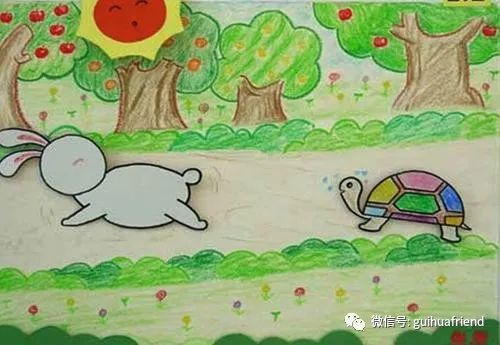
\includegraphics[width = .5\textwidth]{./ch/3.jpg}

\end{figure}



上一次乌龟和兔子赛跑,因为兔子太轻敌了,所以乌龟胜利了。这次兔子吸取了上次的教训,向乌龟宣战。

距离龟兔赛跑第二站还有三天。兔子天天在外面运动。乌龟也不甘示弱,天天在外面运动。时间一天一天的过去了,终于来到了龟兔赛跑第二战的日子,这天赛道旁坐满了观众。

兔子和乌龟站在起跑线上,“砰”,裁判员扣动了发令枪的扳机,兔子“嗖”的一下像火箭一样,冲了出去,而乌龟还在拼尽全力的爬。因为兔子冲得太快了,没有看见前面有个坑 一不小心就掉了进去。乌龟爬呀爬呀,终于超过了兔子,到下坡赛道了,乌龟灵机一动,把头和腿缩进了龟壳里,再往下一滚,咕咚咕咚,乌龟滚了下来,兔子废了九牛二虎之力,才从坑里爬上来。发现被乌龟超过的兔子急急忙忙的追了上来,超过乌龟后,路过了一块萝卜田,兔子看见了水灵灵的萝卜就跑过去,大口大口的吃起萝卜来。

过了很久之后,兔子吃饱了,乌龟也在离终点还有一米的地方奋力爬。兔子看见了,连忙跑过来,可是肚子吃的太饱,跑不动,所以乌龟爬到了终点线,乌龟再次胜利了。

经过这次赛跑,兔子懂得了要持之以恒,还说等他锻炼好了,还会来再次宣战。





\vspace{10pt}



作者:四(1)班 吴才俊



指导老师:周瑞



投稿:2021年6月15日



发表:2021年6月16日








                



\vspace{10pt}

\hline



